\documentclass{article}
\usepackage{cite}
\usepackage{amsmath,amssymb,amsfonts}
\usepackage{algorithm}
\usepackage{algpseudocode}
\usepackage{array}
\usepackage{booktabs}
\usepackage{graphicx}

\usepackage{graphicx,xcolor}
\usepackage{tabularray}

\usepackage{textcomp}
\usepackage{comment}
\usepackage{hyperref}
\hypersetup{
    pdftitle={PoCS Research Model}
    }

\begin{document}

\title{Proof of Contract Stake \\ Research Model}

\author{Joby J Reuben \\
Auguth Research Foundation \\
Bangalore, India \\
joby@auguth.org
}

\maketitle

\begin{abstract}

Proof of Contract Stake (PoCS) is an innovative staking system utilizing contract gas history to select block producers. It merges proof-of-work and proof-of-stake, introducing "code-mining" by incentivizing developers to secure the network. Contracts' stake scores depend on age, reputation, and gas use, deterring collusion attacks. PoCS eliminates the "nothing at stake" attack with a non-fungible non-transferable unit of scarcity to stake. A stake accumulation attack in PoCS is time constrained and patterned, which can be easily detected, escalates costs over time, and cannot be expedited with any external resources.

\end{abstract}

\section{Introduction}

The Proof of Contract Stake (PoCS) is an alternative staking mechanism to Proof of Stake that utilizes the history of gas consumption from contracts as a scarce and limited resource. This resource can be staked to elect/select block producers. PoCS introduces a hybrid proof-of-work and proof-of-stake model, offering an environmentally sustainable solution that can be relied upon for a public blockchain's network security. This consensus model focuses on developers, providing them with an incentive mechanism for contributing to network security.

Contract storage fields are expanded to allow the validator's information to be stored with specific conditions where each contract's stake score is determined based on various parameters, including its staking age, reputation, and total metered gas consumption. These factors can be delegated to a chosen validator by the contract's owner.

One noteworthy achievement of the PoCS consensus model is its ability to eliminate the "nothing at stake" problem. This is achieved by maintaining non-fungible and non-transferable stakes, similar to PoW systems. However, PoCS introduces a significant attack vector known as the "collusion attack", which allows validators to artificially inflate gas consumption. Collusion attacks occur when a block author intentionally increases the scarcity of a staked contract, either owned by themselves or a partner, and includes malicious high gas transactions to gain an unfair advantage.

To counter this issue, PoCS incorporates a built-in contract reputation model that is directly proportional to the stake. This approach ensures that attempting to attack the network becomes increasingly costly over time, making it impractical and unprofitable compared to honest block production. Consequently, validators are motivated to avoid the risk of slashing and malicious activities.

PoCS can bring in public good projects where Smart Contract Developers within this ecosystem can benefit from PoCS staking by availing an alternative contract staking business model as opposed to traditional token-based/platform fee models.

\section{Goals}

\begin{enumerate}
    \item \textbf{Innovate Security Approach:} PoCS introduces a novel method for enhancing blockchain security through "code mining". This novel approach enables any contract to contribute to security by possessing a specific and unalterable "stake score".
    \item \textbf{Revolutionize Business Methods:} PoCS aims to reshape how blockchain-based businesses generate income. By implementing the concept of staking programs, as opposed to relying solely on traditional tokens or platform fees, PoCS offers an alternative avenue for projects built on these networks to thrive and avoids scams and rug-pulls.
    \item \textbf{Reward Developers:} Incentivizing developers is a central aspect of PoCS. By offering rewards to developers who stake their contracts with validators (the entities responsible for validating transactions on the blockchain), PoCS cultivates a stronger developer community.
    \item \textbf{Spread Out Ownership:} PoCS tackles the issue of concentrated control by introducing a unique form of stake that can't be divided or transferred like regular tokens. This approach broadens ownership and minimizes the impact of market conditions.
    \item \textbf{Keep Control Safe:} PoCS introduces a mechanism that empowers individuals to contribute to network security without giving up control of their assets to validators. This strategy mitigates the risk of potential attacks stemming from excessive validator influence.
    \item \textbf{Trustworthy Contracts:} PoCS prioritizes the creation of reliable smart contracts. By enabling users to choose contracts with established reputations for security and reliability, PoCS bolsters user confidence in interacting with the blockchain.
\end{enumerate}

\section{Extended Details on PoCS}

\subsection{Security equals Scarcity}

Consensus models that secure a possibly dishonest, distributed, untrusted network rely on a scarcity element as their sole vector to protect from various attacks. Proof of Work (PoW), notably secures the \href{https://bitcoin.org/bitcoin.pdf}{Bitcoin Network}, the scarce resource is the \textit{computational capacity} $(c)$ to compete in producing blocks $(L)$. This concentration of the scarce resource makes it costlier for attackers to replay and overpower the network $(F)$ compared to the current hardware available to them.

\[
Security(PoW) = g\left(\frac{c}{F},\frac{1}{L}\right)
\]

With Proof of Stake (PoS), the scarce resource relies on the network's cryptocurrency itself, where validators are required to \textit{lock up a fungible unit} that can be transferred between various accounts. This vulnerability to concentration into a few actors also makes it economically harder (though not impossible) due to its value $(v)$ being tied to the market and its liquidity $(l)$ being scarce.

\[
Security(PoS) = g(v,l)
\]

Therefore, in both PoW and PoS cases, the security of the network is intrinsically tied to the \textbf{scarcity} of the resource, ensuring a robust and resilient decentralized system that can be trusted by its users. However, the increasing adoption of PoS in upcoming blockchains has led to a surge in new native tokens with higher liquidity and lower market value with potential restrictions necessitating token sales/offerings. This raises concerns about centralization, distribution, legal issues, and loss of network independence to a centralized foundation.

Additionally, due to the \textit{environmental inefficiency} of currently available alternative PoW systems using ASIC resistant hash-functions \& even CPU-mining algorithms like \href{https://github.com/tevador/RandomX}{RandomX} encourages miners to infect PCs with Trojan malwares. There is a growing need for a hybrid PoW and PoS consensus model that provides non-carbon emissive computational power with staking. This hybrid approach can potentially facilitate a fully decentralized and publicly operable network with better use cases and global acceptability.

Proof of Contract Stake (PoCS) relies on the \textbf{history of computational units} $(c$ as gas units, $t$ as time$)$ to be used for staking. This facilitates an arbitrary innovation to make an \textit{individual contract's immutable history a scarce resource}.

\[
Security(PoCS) = g(c,t)
\]

Similar to a mined currency through block rewards which are used for staking, PoCS's \textit{non-fungibility} makes it a better alternative to both PoS and PoW. The scarce element of PoCS prevents security from being concentrated and provides a much more decentralized zero-trust network, capable of being accepted by anyone around the globe, as there is no need for specialized hardware or market accumulation.

PoCS Non-Fungibility can be expressed as,

\[
PoCS \rightarrow c(Val_A) \cap c(Val_B) = \emptyset
\]

A wider distribution with lower concentration indicates lesser concerns for lacking security. Conversely, higher concentration suggests that actual security is not reliant on a scarce resource but rather an available one, with the opportunity for attacks or collusion with dishonest parties. Proof of Stake (PoS) systems encourage the concentration of the scarce resource (staking tokens) over time $(t)$. The staking rewards, compounded over multiple periods, incentivize larger stakeholders to accumulate more tokens, leading to wealth concentration and loss of scarcity.

\[
PoS \rightarrow Reward = k \times (a + \Delta a)
\]

where, $a$ is the stake and $\Delta A = n \times unitValue$

\[
PoCS \rightarrow \Delta c = k \times t(U(C))
\]

Unlike PoS, PoCS doesn't compound the stake and doesn't allow validators to accumulate or inflate the scarce resource by influence. Contracts $(C)$ that undergo high usage $(U)$ by users will be provided with higher staking scores that can be saturated by newer contracts and their usage history. With PoCS the cost of acquiring the scarce resource is tied to block time $(t)$ and transaction fee cost that cannot be accumulated compared to PoS's tokens liquidly available to accumulate instantly in an open market that is subject to concentration and inequality.

\subsection{Eliminating Nothing at Stake Attack}

PoCS challenges the likes of PoS consensus by eliminating the "nothing at stake" attack that encourages validators to have nothing to lose by staking on multiple, potentially conflicting, blockchain branches without incurring significant costs or consequences. This attack arises due to reusing the balances with multiple validators, which cannot be burnt, to reimburse stakers. This is due to the fact that PoS uses a fungible unit that doesn't function similarly to mining hardware, where the computation done cannot be reused.

In PoCS (Proof of Contract Stake), a validator's total stake is automatically linked to the network's transaction history, and validators won't have the independence selectively to choose stakers and their scarce resource to participate in the block authoring process. If stakers decide to delegate their contracts to a different validator, their \texttt{staking age} and \texttt{gas consumption} will be purged to prevent the reuse of scarce elements which is vital for network security. Since PoCS's scarce element "History of gas consumption" is a \textbf{non-fungible, non-transferable} resource that is only used to maintain network security and to receive staking rewards, it doesn't necessarily need to be reused like native balance and purges when \texttt{delegateTo} (delegated to a validator) updates.

If the probability of a branch being selected increases, it will increase the chances of motivation to split stakes between multiple branches. After split-branch selection probability $\mathbb{P}'(A)$ should be lesser than or equal to $\mathbb{P}(A)$, the before split-branch selection probability, to avoid and eliminate the "Nothing at Stake" problem.

\textbf{In the basic PoS model:}

\begin{itemize}
    \item Probability of branch $A$ being chosen: $\mathbb{P}_A = \frac{v}{V}$, where $v$ = Number of validators staking on branch $A$ and $V$ = Total number of validators in the network.
    \item Probability of branch $B$ being chosen: $\mathbb{P}_B = \frac{w}{V}$, where $w$ = Number of validators staking on branch $B$.
\end{itemize}

\textbf{When validators can split their stake:}

Updated probability for branch $A$:

$$\mathbb{P}'_A = \frac{v}{V} + \frac{w}{2V}$$

Updated probability for branch $B$:

$$\mathbb{P}'_B = \frac{w}{V} + \frac{v}{2V}$$

Motivation to split stake,

$$\mathbb{P}'_A = \frac{v}{V} + \frac{w}{2V} > \frac{v}{V} = \mathbb{P}_A$$

In PoCS, once the staker decides to switch validators, their previous stake (gas consumption) becomes zero. By ensuring that the \textit{stake is strictly tied to the validator} and is \textbf{reset to zero} when the validator is changed, we eliminate the possibility of validators having "Nothing at Stake" when multiple branches exist.

\textbf{Case Scenarios:}

\begin{itemize}
    \item \textbf{Case 1}: Staker on Branch $A$ $(S_A > 0)$ and changes validator: $S_A=0 \rightarrow S_B>0$
    \item \textbf{Case 2}: Staker on Branch $B$ $(S_B > 0)$ and changes validator: $S_A>0 \rightarrow S_B=0$
    \item \textbf{Case 3}: Staker on Branch $A$ $(S_A > 0)$ and does not change validator: $S_A>0 \rightarrow S_B=0$
    \item \textbf{Case 4}: Staker on Branch $B$ $(S_B > 0)$ and does not change validator: $S_A=0 \rightarrow S_B>0$
\end{itemize}

This property \textit{prevents} the staker from having multiple active stakes on different branches simultaneously, eliminating the Nothing at Stake attack and avoiding reusability of stake in different branches. In simple terms, since validators have nothing to influence, choose, or modify the behaviors of their stake, they cannot carry out a split-branch approach.

\subsection{Non-Custodial Stake}

With PoS, there is a risk of \textbf{custodians} ($C_r$) when validators are delegated by holders of the native token. Some of the risks include:

\begin{enumerate}
    \item \textbf{Slashing risk} ($s$): If the exchange's validator node is found to be misbehaving, it may be slashed, which means that the exchange will lose some of the tokens that it is staking.
    \item \textbf{Manipulation risk} ($m$): The exchange could potentially manipulate the staking process in order to benefit itself, at the expense of the users. For example, the exchange could choose to stake the tokens on low-risk validators, even if this means that the users will earn fewer rewards.
    \item \textbf{Loss risk} ($l$): The exchange could lose the tokens that it is staking due to a security breach or other incident.
\end{enumerate}

$$PoS(C_r) = s + m + l$$

$$PoCS(C_r)=s$$

In PoCS, the contract deployer is provided with the non-custodial model to register his \texttt{delegateTo} address of the validator and the validator holds no authority over the staked contracts, thus providing a non-custodial model with only slashing risk associated with lesser returns on rewards by validators not frequently chosen for block production.
The integration of Proof of Contract Stake (PoCS) introduces a potential attack vector. In the initial stages of a network incorporating PoCS, there exists a vulnerability where validators may collude with contracts staked to themselves, employing malicious code with the intent to *escalate gas consumption* (PoCS's scarce unit) and enhance their chances of authoring blocks. Although some block candidate announcing models like Polkadot's BABE consensus effectively avoid consecutively allowing validators with the largest stake holdings to produce blocks, many algorithms still rely on the *largest stakeholder* model. Moreover, **collusion attacks** can be executed when gas prices are low, taking advantage of the market value associated with the native token charged for transaction fees.

\subsection{Contract Reputation}

The integration of Proof of Contract Stake (PoCS) introduces a potential attack vector. In the initial stages of a network incorporating PoCS, there exists a vulnerability where validators may collude with contracts staked to themselves, employing malicious code with the intent to \textit{escalate gas consumption} (PoCS's scarce unit) and enhance their chances of authoring blocks. Although some block candidate announcing models like Polkadot's BABE consensus effectively avoid consecutively allowing validators with the largest stake holdings to produce blocks, many algorithms still rely on the \textit{largest stakeholder} model. Moreover, \textbf{collusion attacks} can be executed when gas prices are low, taking advantage of the market value associated with the native token charged for transaction fees.

As we envision implementing a fully arbitrary fee model for validators in the future via \textit{Barter Gas Protocol} (Will update once the discussion is live), allowing them to charge \textit{local fees} instead of adhering to a consensus-accepted fee structure, the same collusion vulnerability arises. This vulnerability enables the execution of artificially inflatable high gas transactions by colluded contracts, utilizing valueless tokens or arbitrary fee-accepting proofs that do not yield immediate profits for the validator but aim to secure future block authoring opportunities with \textit{artificially inflated stakes}. However, over time, these various collusion methods will incur increasing costs, as the benefits of accepting legitimate transactions will become more \textbf{profitable} than the cumulative gains from artificially inflating gas transactions to secure future block authorship.

\begin{table}[h]
    \centering
    \renewcommand{\arraystretch}{1.5}
    \setlength{\tabcolsep}{10pt}
    \begin{tabular}{|p{0.5\textwidth}|p{0.5\textwidth}|}
        \hline
        \textbf{Claim} & In initial low-value token networks $\mathbb{P}_{collusion}$ is higher \\
        \hline
        \textbf{Assumption 1:} & Probability of Block Selection is Proportional to Validator's Stake. $bs =$ block selection \\
        $\mathbb{P}_{bs} (V_n) = k \times St$ & \\
        \hline
        \textbf{Assumption 2:} & Probability of Collusion is a Function of Fee Token Value. \\
        $\mathbb{P}_{collusion} = f(Val)$ & \\
        \hline
        \textbf{Assumption 3:} & Collusion Probability Decreases with Increasing Token Value. \\
        $\mathbb{P}_{collusion} = \frac{k'}{Val}$ & \\
        \hline
    \end{tabular}
    \caption{Probability assumptions for collusion in low-value token networks.}
    \label{tab:collusion_probabilities}
\end{table}

In the context of L1s and generalized state machines, it remains \textit{challenging} to completely prevent the deployment of gas-consuming malicious contracts. Although validators can diligently act to avoid such contracts when a trusted audit entity provides a \textit{blacklist} of contract IDs for exemption from mempools, these solutions rely on trust and do not guarantee a fully trustless system capable of avoiding code deployments \& executions with harmful parameters.

To address this, we propose the implementation of a \textbf{trustless contract reputation score}, which can impact the stake score associated with a contract by evaluating its reputation through \textit{recurring transactions in consecutive blocks}. This approach aims to provide a more robust and decentralized method for assessing the trustworthiness of contracts without relying on external trust-based measures.

\begin{equation}
R(account_{id})  = \sum_{i=1}^{n} R_i
\end{equation}

\begin{equation}
R_i = \begin{cases} 
     1, & \text{if contract's tx is in the } i^{th} \text{ block} \\
     0, & \text{otherwise}
\end{cases}
\end{equation}

An $account_{id}$ containing \texttt{Reputation Score} ($R$) mapped with \texttt{recentBlockHeight} ($r$), when a transaction executes in $n$ as \texttt{currentBlockHeight}, :

\begin{equation}
R(account_{id}) \leftarrow R + \begin{cases}
    1, & \text{if } n > r \\
    0, & \text{otherwise}
\end{cases}
\end{equation}

\begin{equation}
r \leftarrow \begin{cases}
    n, & \text{if } n > r \\
    r, & \text{otherwise}
\end{cases}
\end{equation}

PoCS's contract reputation trustlessly evaluates a contract's reputation based on its usage history but also avoids Collusion attacks by keeping the reputation increment \textbf{restricted to time} (block height).


\subsection{Contract Stake Score}

In PoCS consensus, the \texttt{stake\_score} of a contract plays a crucial role in determining the proportion of the overall stake delegated to validators contributed by all contract owners. The stake score is a \textit{deterministic value} calculated based on several factors, such as the contract's \texttt{gas\_consumption} ($g$), \texttt{reputation} ($R$), and \texttt{recentBlockHeight} ($r$). By considering these elements, the system can effectively prevent various collusion attacks and promote a fair distribution of rewards to staked contract owners. This approach fosters a trusted network environment, as it incentivizes long-term commitment to the network and ensures that validators and contract developers are duly rewarded for their contributions.

\begin{equation}
\texttt{stake\_score} = \texttt{stake\_score} + (R \times g)
\end{equation}

\textbf{Claim}: The Stake Score formula improves randomized results, competition, long-term commitment, and fair reward distribution, and prevents collusion with malicious intent.

\[
\begin{array}{|c|p{8cm}|}
\hline
\textbf{Property} & \textbf{Proof Statements} \\
\hline
\text{Unpredictable} & Contracts cannot predict the usage of users which influences the gas consumption ($g$). \\
\hline
\text{Competition} & Contracts compete for higher $\texttt{stake\_score}$ by being more active, reputable, and optimizing gas consumption for more users to engage with less economic costs. \\
\hline
\text{Long-Term Commitment} & A $\texttt{stake\_score}$ is influenced by reputation ($R$), hence long-term commitment is encouraged. \\
\hline
\text{Fair Reward Distribution} & $\texttt{stake\_score}$ is based on genuine usage, reputation, and efficiency, not just delegated stake. \\
\hline
\text{Scarcity Dilution} & Contracts with positive attributes can compete effectively with other contracts, diluting scarcity concentration. \\
\hline
\end{array}
\]

Let $\mathbb{P}_{\text{collusion}}$ be the probability of successfully executing a collusion attack to increase gas consumption for future block authoring by a malicious contract. The Stake Score ($\texttt{stake\_score}$) with \texttt{reputation} and \texttt{stake age} prevents artificial inflation of the Stake Score, making $\mathbb{P}_{\text{collusion}}$ lower over time. With reputation tied to stake, a collusion attack requires cooperation from \textbf{2/3 network validators} to execute malicious contracts, making it highly unlikely in a PoCS network. Therefore, $\mathbb{P}_{\text{collusion}} < \mathbb{P}_{\text{honest}}$, where $\mathbb{P}_{\text{honest}}$ is the probability of honest block authoring.

\subsection{External Call Monetization}

To ensure the validity of Proof of Contract Stake (PoCS) in terms of \textbf{code mining} and incentivizing every individual innovation, the inclusion of external cross-contract calls becomes essential. Within a blockchain transaction, the flexibility exists to contain \texttt{public} and \texttt{private} calls or execute functions that can modify the contract's \textit{state} while encompassing multiple \textit{external contract calls} executed within the same transaction. While the \texttt{gas\_consumption} (scarce unit in PoCS) metric represents the total gas utilized by the transaction, it should be further broken down or \textit{dissected} to reflect the gas consumed by the \textit{externally called contracts} also.

\subsection{Saturable Governance}

On-chain governance in PoS relies on the Chain's native token-holders voting to accept \textit{Improvement Proposals}, thus amending the change via a \textit{manual hard fork} or forkless runtime upgrades in the context of Substrate Standalone Chains / Polkadot's Parachains. This democratic voting has led to positive changes in \textit{Off-chain governance} such as Bitcoin and \href{https://ethereum.org/governance}{Ethereum}, involving consensus from various node providers, miners, stakeholders, etc. However, it also has significant issues, which PoCS aims to solve.

Many PoS Chains that undergo Initial Coin Offerings (ICO) have distributed their token shares mainly to the \textit{foundation} behind the project and whitelisted early investors, while a minority share is airdropped or sold to retail investors who believe in the project's success.

\[
\text{Distribution} = \text{Foundation} + \text{Insiders} > \text{Retail}
\]

\[
V(t, p) \in \{ 0, 1\}
\]

where \(V(t, p)\) represents the voting decision of token holder \(t\) on Improvement Proposal set \(p\).

Philosophically, Smart Contract developers who build on top of these PoS L1 chains should have a major say in what the protocol should upgrade, in order to drive in with the upgrades amended to their projects as well. Since each vote in PoS consensus has an \textit{unequal weight}, these Improvement Proposals influenced by large token holders such as the L1 project's creators, and early investors, make the proposal amendment \textit{centralized}.

In PoCS, stakeholders, i.e., the deployers of contracts holding a \textit{definitive stake score}, can propose Improvement Proposals and vote for existing proposals with their \textit{stake as weight}. With PoCS, there comes inclusivity to developers who build smart contracts on top of the blockchain.

\[
U(SS_{Main_{id}},G) \in \{ 0,1 \}
\]

where \(U(SS, G)\) represents the influence of the Smart Contract developer on the Improvement Proposal \(G\).

This requires any proposer to actively work on the PoCS Chain, where their \texttt{reputation} of contracts succeeds in the validation to be attested for every proposal. Meanwhile, researchers, by initially deploying a contract and taking the required reputation, can propose changes.

\[
SS_{Main}[C_{id}] > 1
\]

The participation for voting will include active developers who are monetizing their contracts and working on easing gas consumption by periodically updating their contracts \href{https://use.ink/basics/upgradeable-contracts/\#\#replacing-contract-code-with-set_code_hash}{Upgradable Contracts} in the context of Substrate, unlike dormant holders of a cryptocurrency who are hidden from participating in a long, \textit{chores-like} process.

With Substrate's forkless runtime upgrades, these governance decisions involving upgrades can be made useful to \textbf{upgrade run-time automatically} once the voting period ends according to the results on-chain.

\subsection{PoCS \& Block Authoring}

The PoCS module is considered a \textbf{pre-staking module} and does not function as a block author announcement and verification module. Instead, it can collaborate with existing block authoring protocols such as \href{https://wiki.polkadot.network/docs/learn-consensus#nominated-proof-of-stake}{NPoS}-\href{https://wiki.polkadot.network/docs/learn-consensus#block-production-babe}{BABE} in Substrate/Polkadot or a new staking algorithm customized for it, as PoCS does not rely on conventional token-based bonds but utilizes a scoring mechanism. 

In most consensus mechanisms, validators must fulfill a \textbf{minimum token staking requirement}, and nominators/delegators contribute to the selection of validators to produce specific block heights. The PoCS module can identify validators meeting a minimum staking requirement according to its protocol's criteria, based on \texttt{stake\_score} rather than token units, and assign them to the block authority set in accordance with the rules of the block authoring protocol. 

An optimal staking mechanism involves bonding, nominating (delegating), and validating, which are described below to fulfill a PoCS-suitable criterion.

\subsubsection{Minimum Requirements}

Contracts can be bonded similar to locked funds, which requires authorization from the contract deployer. During deployment, the contract can automatically be bonded to the deployer's address themselves at a zero bond value, since bond value can only be increased during calls made to the contract. While the bond can persist with zero value, the nomination or delegation to a validator after contract deployment can possess a certain criterion. 

For updating the delegate information from the default deployer address to a validator address, a minimum requirement can be imposed to avoid unintended attacks; however, contract's stake\_score's minimum value cannot be enforced due to its proportional tie to reputation and gas units. Therefore, a constant \texttt{reputation} requirement, modifiable according to the network's condition, can be imposed while also introducing a common threat that is prevalent in almost every random validator selection algorithm-based public blockchain, counterfeit attacks.

\textbf{Reputation as a minimum requirement} for a bond to be staked or nominated to a validator is similar to a minimum token value's lock-in. Gas costs are spent to call a contract, which is required to increase its reputation, avoiding artificial inflation and thus increasing costs based on the network's performance and reputation criteria. Upon ensuring a contract's reputation fulfills the minimum reputation requirement, the delegate information can be updated, and automated nomination for all epochs is ensured.

Validators' requirements can be tied to the number of contracts they handle as stake/bond. Just as contracts need a certain reputation to nominate a validator, validators must be nominated by a certain number of contracts to initiate validation.

\subsubsection{Counterfeit Attacks}

Similar to token demand's (market price) influence on staking requirements, a higher availability (liquidity) of a stakable asset might require the network's governance to increase the staking requirement and vice versa when there is higher demand. In PoCS, updating minimum reputation and the minimum contract bonds based on the network performance or other criteria—such as the cost of creating counterfeit contracts and attempting to increase their reputation for staking purposes—can increase the cost, making such attacks costlier to carry out compared to honest production. 

Adopting a largest stake-based block authoring protocol emerges as the most effective alternative to thwart counterfeit attacks. This approach eliminates minimum staking requirements and dynamically adjusts to network conditions. Imposing specific constants as requirements necessitates analysis and updates by a central entity, introducing complexity and time consumption.

\subsection{Suspension as Penalty}

Penalties can be imposed upon validators who engage in activities that can be construed as malicious attacks conducted by network nodes. Such actions can result in the suspension of a validator for a specified number of blocks, placing them in an idle position. As the Stake Score is both non-fungible and non-transferable, rendering it unusable outside the staking environment, reducing or slashing it is ineffective in mitigating the severity of attacks. Suspending a validator proves to be an effective approach to penalize node operation costs and to notify bonded contract owners to reconsider their validator choices in order to prevent their stake from becoming idle.

The seriousness of a dishonest act is assessed by multiplying the gravity of the offense by the \texttt{warmTime}, which can be set at \( x \) blocks. For example, a 6-second block time, with an average of \( 75,000 \) blocks, translates to an average duration of approximately 5 days. The \texttt{warmTime} serves as a defined period for any actions necessitating a gradual adjustment or preparation and can be used for multiple scenarios.

\subsection{Majority Stake Attack}

Acquiring a stake in PoCS requires the payment of a gas fee to execute a contract or set of contracts that are staked with the attacker's validator. This process involves convincing other block authors to validate the transactions following an explicitly visible attack transaction, repeated over a certain period of time. Since PoCS does not involve the accumulation of native balance (native tokens), these attacks can be easily detected by general watchers, instructing honest block authors for their benefit by rejecting such transactions.

The accumulation of stake attack represents a collusion attack without a validator's participation in it, wherein attackers artificially inflate their stake by compensating honest validators to include their transactions in their blocks. As the inflation of stake cannot be acquired from an external market like tokens, this attack is subject to a time constraint and becomes saturated by other transactions with its uncertain reputation (uncertain honest transactions) if the attacking transaction is not the sole transaction included in a block.

There are two primary methods through which a stake accumulation attack can occur in PoCS:

\begin{enumerate}
    \item Honest block authors accepting a stake accumulation attack transaction or transactions in which a contract or set of contracts transacts by paying fees for the entire period of blocks that will last for weeks, effectively halting the chain. This is similar to an entire network accepting an attack to take place, which is self-destructive and disincentivizes forward movement. Hence, this attack is a potential but implausible event. With a set of multiple contracts, this attack can be identified, as all the colluded contracts would have been staked to a single validator or a few, patterned in consecutive blocks.
    \item The attacking party accumulates stake through a transaction that lacks a discernible pattern. This transaction is included in a block alongside multiple other transactions. Given a gas limit cap per block or under a block time, such a transaction could possess a high gas limit. With this approach, the attack can take a long period of time and be unachievable due to other contracts' stake score saturation on the total network stake during the attack period.
\end{enumerate}

To possess a 51\% stake, the validator needs to stake:

\[
x=\frac{\text{current network stake} \times 0.51}{0.49}
\]

To avoid the attack surface, validators can prioritize transactions that have a higher reputation as opposed to newly created contracts with a lower reputation. Hence, validators' priority of transactions should not focus entirely on the transaction's gas price but also on identifying the reputation of the transaction via its calling contract's reputation.

\subsection{Possessive Attacks}

Possessive attacks occur when validators selectively choose specific transactions to artificially increase their nominator bond values. This behavior can lead to unfair advantages in staking and disrupt the integrity of the PoCS mechanism. 

Addressing this issue is critical to maintaining a decentralized and fair staking environment. The upcoming \textit{BarterGas Protocol} aims to resolve this vulnerability by ensuring a more balanced and transparent transaction selection process, preventing validators from exploiting selective staking strategies.

\subsection{Limitations}

The limitations of Proof of Contract Stake (PoCS) are primarily rooted in its design and application. PoCS relies on assigning a \textit{scarcity resource} for staking based on an individual contract's \textit{history of usage} within a specific time frame, which leads to the following key limitations:

\begin{enumerate}
    \item \textbf{Dependency on Smart Contract Blockchains}: PoCS can only be effectively utilized on a smart contract-enabled blockchain. Since it relies on monitoring and evaluating the usage of individual contracts, it requires the underlying blockchain to support \textit{smart contracts}. This limitation restricts its applicability to platforms that do not have smart contract functionality.
    \item \textbf{Limited Applicability to Non-Contract-based Transactions}: PoCS's design is tailored explicitly for smart contract interactions, which means it may not be suitable or applicable for blockchain use cases that primarily involve \textit{simple transactions} without smart contract involvement.
\end{enumerate}

\subsection{Future Work}

In terms of future work, our primary focus will be on the development of a fee model named \textit{Barter-Gas}, designed for implementation on public blockchains. This model introduces an additional fee transaction as a batch process, allowing expected contract state updates to be taken as fees with flexible benefits. Notably, this system enables validators to accept these benefits as fees, streamlining a blockchain to be adopted globally without reliance on a native token for fees, since PoCS replaces the security reliance of tokens in a public smart contract network.

Furthermore, our ongoing research will address potential attack vectors associated with the Proof of Contract Stake (PoCS) mechanism. We will also explore practical implementation models for PoCS concepts, contributing to the advancement of public blockchains.

\section{PoCS Simulations (Ethereum PoCS)}

We will simulate PoCS on Ethereum transaction history and analyze how PoCS would have behaved if Ethereum had implemented PoCS from its genesis block. The results aim to provide insights into its impact on staking dynamics.

Ethereum history was queried and downloaded from \href{https://bigquery.cloud.google.com/dataset/bigquery-public-data:crypto_ethereum}{BigQuery crypto.ethereum}. Input Table: Transactions.

The simulation scripts that generate the following charts can be found in the source repository of this research article.

\subsection{Ethereum on PoCS Stake Supply}

We simulate the total network stake supply based on Ethereum's transaction history, providing an overview of the network's stake per time period (1 month) and its supply curve. Due to the uncertainty of staking age, we assume that contracts have not changed validators since their creation.

\begin{figure}[h]
    \centering
    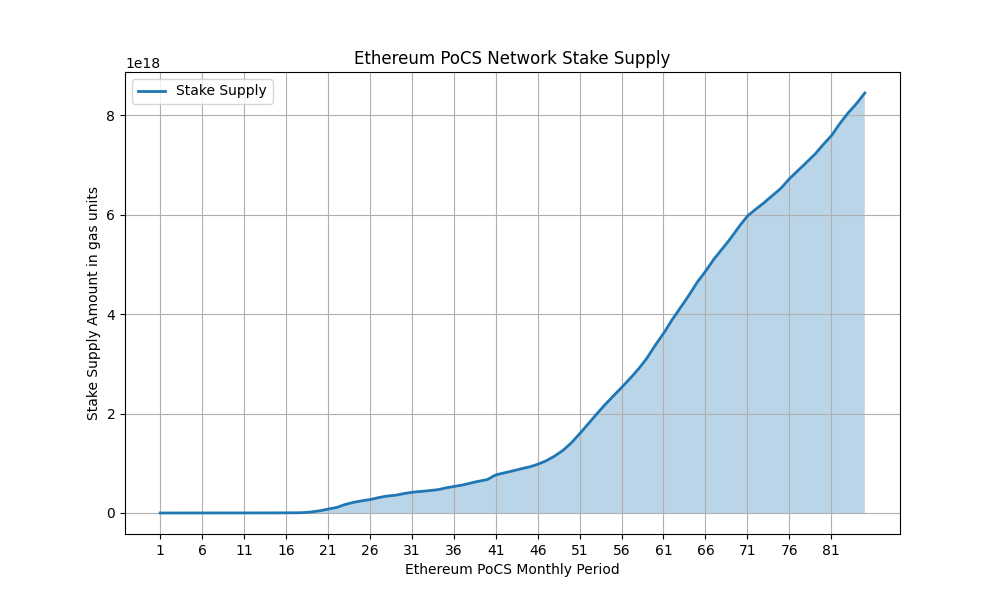
\includegraphics[width=\textwidth]{./assets/eth-pocs-supply.png}
    \caption{Ethereum PoCS Network Stake Supply}
\end{figure}

\begin{itemize}
    \item The simulation results illustrate Ethereum PoCS's transaction landscape up until the beginning of the 20th month, covering a span of over 1.6 years. During this period, Ethereum predominantly featured simple balance transfers rather than contract calls. PoCS consensus is optimally suited for blockchains dedicated to contract execution, where complex interactions outweigh simple value transfers.
    \item A significant shift occurs around Month 50, marking the beginning of Ethereum’s fourth year. During this phase, contract transaction stake scores exhibit a recurring pattern of doubling each month. This surge correlates with the simultaneous rise in gas consumption and the accumulation of contract reputation within the Ethereum PoCS simulated ecosystem.
    \item This analysis is based on a simplified simulation using available metrics—gas consumed and contract reputation. However, the uncertainty surrounding stake age introduces an element of unpredictability. This uncertainty enhances security by obfuscating the exact costs and timeframes required for a malicious contract to inflate a 51\% stake.
\end{itemize}

\subsection{Staking Uniswap on Ethereum PoCS}

We simulate Uniswap V1, V2, and V3 running on Ethereum with Proof of Contract Stake (PoCS) and analyze the network-to-stake ratio. This provides insights into the total stake held by Uniswap developers compared to Ethereum PoCS's total network stake at specific time slots (typically every 1 month). Due to the uncertainty of staking age, we assume that contracts have not changed validators since their creation. Additionally, monthly staking rewards are estimated under the assumption that the validator sample size is large (following the Law of Large Numbers Probability), given that block author selection and stake rewards involve inherent uncertainty.

\begin{figure}[h]
    \centering
    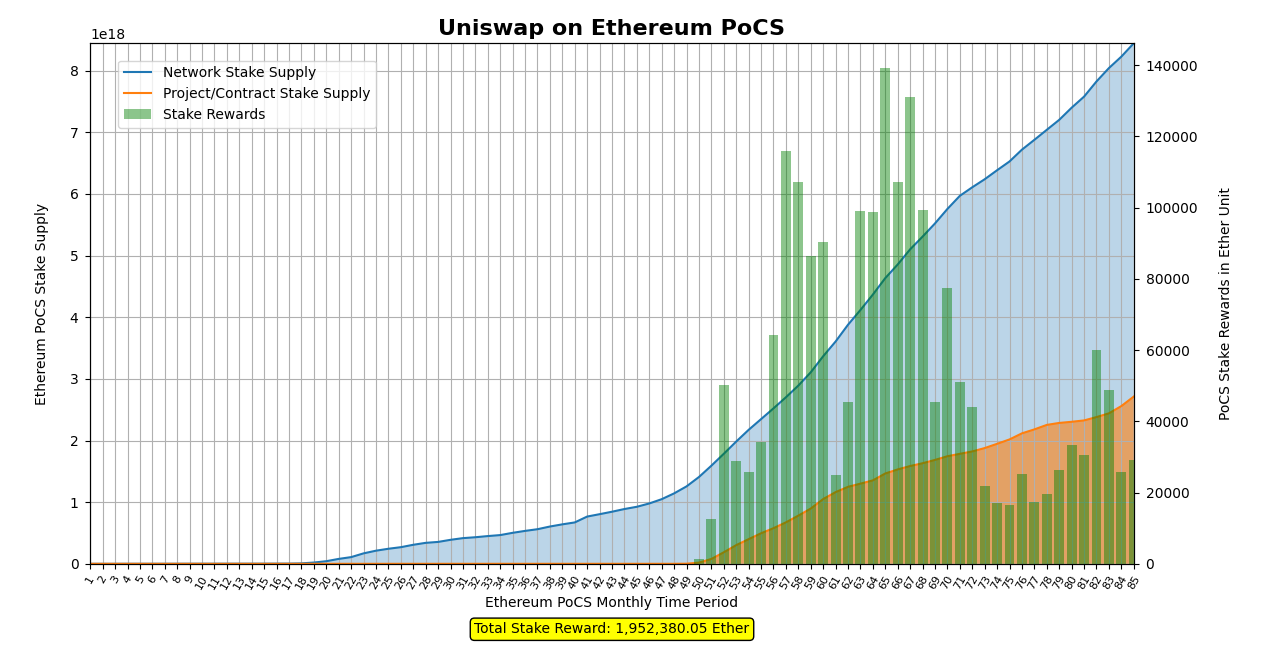
\includegraphics[width=\textwidth]{./assets/uniswap-pocs.png}
    \caption{Uniswap - Ethereum PoCS}
\end{figure}

Readers can explore staking insights for various contract addresses and projects by using the \href{https://github.com/auguth/dot_org/tree/gh-pages/assets/pocs/simulation/pocs}{simulation scripts}.

\begin{itemize}
    \item Uniswap, being a dominant application on the Ethereum platform utilizing the PoCS consensus mechanism, may have generated an estimated income of approximately 2 million Ether to date (equivalent to 3 billion USD).
    \item As of now, the influx of additional dApps saturating the Ethereum ecosystem has resulted in Uniswap falling below the 51\% stake threshold. This suggests that other dApps hold relatively lower stakes, reducing the risk of a majority stake attack on the most widely used dApp.
    \item There is inherent uncertainty regarding stake age. In our analysis, we assume that Uniswap contracts have not altered their validators, thereby preventing any loss of stake. However, in real-world conditions, contracts may modify their validators, potentially affecting their stake scores.
    \item With Ethereum employing the PoCS mechanism, Uniswap consistently generates an income exceeding 20,000 Ether per month. At an estimated average conversion rate of 1 Ether to 1000 USD, this equates to approximately 20 million USD per month, accumulating to around 240 million USD annually. This estimation does not factor in development and operational costs. Given that Uniswap Labs operates with fewer than 50 employees, this level of profitability within the Ethereum ecosystem exceeds initial expectations.
    \item It is important to recognize that these dynamics can change due to various factors, such as shifts in the blockchain ecosystem and fluctuations in transaction fees.
\end{itemize}

\subsection{Ethereum PoCS Majority Stake Attacks}

To simulate a collusion attack, we introduce attack transactions into Ethereum’s transaction history discreetly. These attack transactions, along with their gas usage, are derived from the existing contract transactions’ gas consumption, which contributes to the network’s stake supply in each block. By integrating these attack transactions alongside regular contract transactions, we construct a transaction history that models a colluded scenario. The gas consumption of attack transactions per block, within a monthly range, is controlled by a parameter denoted as \( K \), representing the proportion (\( x \) percent) of gas drawn from the sum of contract transactions within a specific block.

In real-world scenarios, attack transactions may be detected and rejected by block producers to safeguard their stake scores. Due to unpredictable patterns, attempting collusion is likely unfeasible for more than 20\% of transactions per block. For this simulation, we consider attack scenarios at both 10\% and 20\% of blocks and analyze the Ethereum Proof of Contract Stake (PoCS) results. The goal is to determine the point in the monthly timeline when the attack becomes unviable (i.e., fails to reach a 51\% stake) due to the saturation of legitimate transactions.

While accumulating native tokens in Proof of Stake (PoS) chains is permitted and Proof of Work (PoW) allows for centralized mining pools, PoCS provides a viable mechanism to prevent attack transactions. Additionally, it enforces a time constraint that makes such collusion attempts increasingly impractical over time.

\subsubsection{Ethereum PoCS 10\% Block Collusion Attack}

\begin{figure}[H]
    \centering
    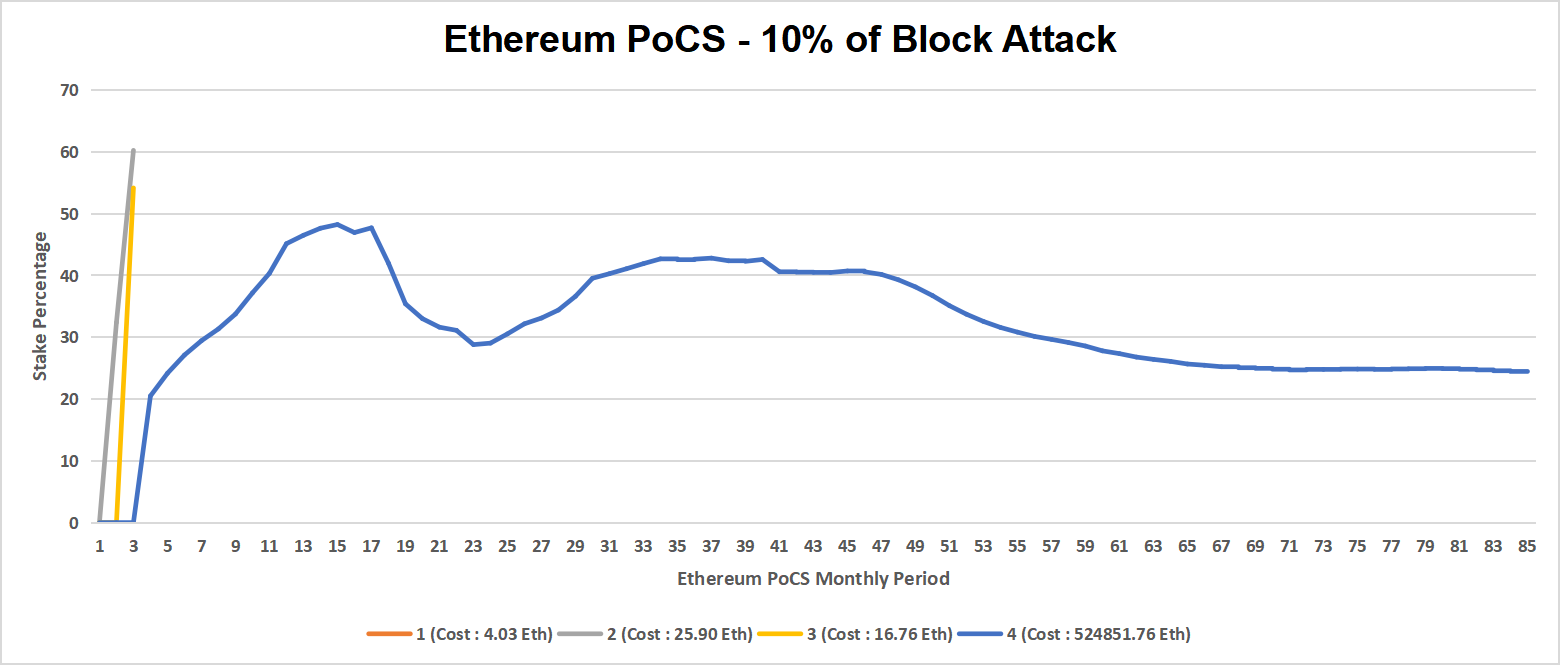
\includegraphics[width=\textwidth]{./assets/10-of-block.png}
    \caption{10\% block collusion attack - Ethereum PoCS}
\end{figure}

\begin{itemize}
    \item The prevalence of primarily simple balance transfer transactions during Ethereum's initial months limits the accrual of stake supply, making PoCS unsuitable due to insufficient stake saturation.
    \item Observing the simulation outcomes, even with an intrusion of attack transactions constituting 10\% of all blocks, commencing from the fourth month, it remains unfeasible for the attacker to attain a 51\% stake.
    \item This underscores the efficacy of PoCS in introducing a time-constraint element. This mechanism effectively safeguards the network from attackers, even when subjected to a 10\% block attack, due to the limitations imposed on the time required to amass a significant stake.
\end{itemize}

\subsubsection{Ethereum PoCS 20\% Block Collusion Attack}

\begin{figure}[H]
    \centering
    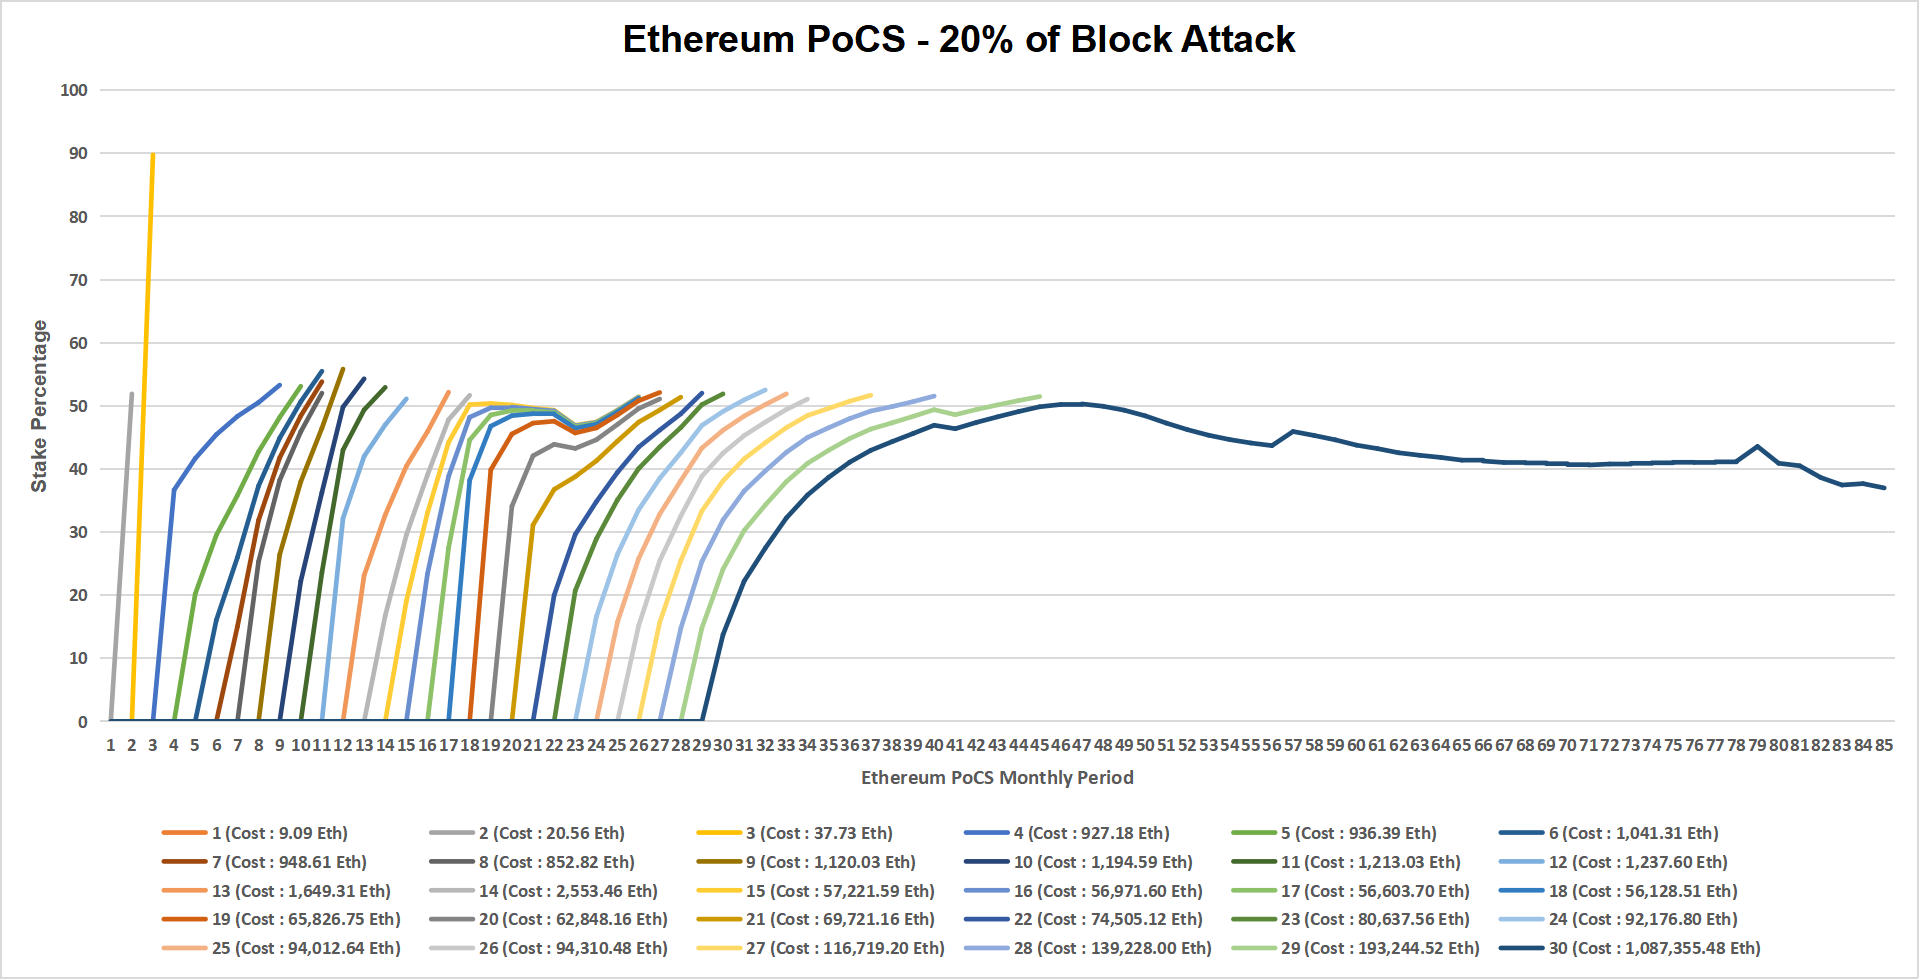
\includegraphics[width=\textwidth]{./assets/20-of-block.png}
    \caption{20\% block collusion attack - Ethereum PoCS}
\end{figure}

\begin{itemize}
    \item Executing a 20\% block attack presents substantial challenges due to the blockchain's pattern recognition mechanisms. Despite this, a simulation of the outcomes can be presented.
    \item Through the simulation, it becomes evident that post the 30th month, executing a 20\% block attack becomes inviable. This is attributed to the saturation of forthcoming blocks, leading to a consistent reduction in the attacker's stake. Despite a constant influx of attack transactions, the attacker's stake diminishes over time.
    \item An attack attempting to secure a stake ranging from 30\% to 100\% faces numerous obstacles such as validator consent, stake age, etc. Higher transaction fees and the resistance of block producers to entertain attack transactions to safeguard their stake and influence in block production act as deterrents.
    \item The simulation results unequivocally demonstrate that attacks initiated from a specific month follow through upcoming months to successfully accumulate the 51\% stake, even in scenarios where simulated attack transactions are persistently included in every block. Providing time for predictability empowers the network to identify and mitigate attacks.
    \item Within the currently available existing consensus models, the detection and reversal of stake accumulation attack transactions, along with the parties orchestrating stake accumulation, are intricate, probabilistic tasks that may involve false positives. Resolving such instances would necessitate a comprehensive hard fork to the chain that impacts all non-attack transactions. The implementation of Proof of Contract Stake (PoCS) effectively counters such potential scenarios, as illustrated by the simulation results.
    \item Notably, since the attack operates by compensating validators through fees, the feasibility of the attack is also contingent on the value of the native token or the designated fee-paying token(s). Fluctuations in token value directly impact the viability and cost of executing the attack.
\end{itemize}

\end{document}
